\documentclass[a4paper,12pt]{article}

% Need \centerdot
\usepackage{amssymb}

% Set margins
\usepackage{geometry}
\geometry{
  top=1.0cm,            % <-- you want to adjust this
  inner=1.5cm,
  outer=1.5cm,
  bottom=1.0cm,
  headheight=3ex,       % <-- and this
  headsep=2ex,          % <-- and this
}

% No page numbers
\pagestyle{empty}

% Set paragraph indent to 2.2mm, even first
\usepackage{indentfirst}
\setlength{\parindent}{2.2mm}

% Image support
\usepackage{graphicx}

% Need \XeLaTex logo
\usepackage{xltxtra}

% Set font to Garamond
\usepackage{fontspec}
\setmainfont[Numbers=OldStyle,
	     Scale=1.05,
	     ItalicFont={Adobe Garamond Pro Italic},
             BoldFont={Adobe Garamond Pro Semibold}
            ]{Adobe Garamond Pro}

% Set section to MidnightBlue with horizontal rule
\usepackage[dvipsnames,usenames]{color}
\usepackage[explicit]{titlesec}
\titleformat{\section}[display]{\Large\color{MidnightBlue}}{\thetitle}{1em}{#1}[{\titlerule}]

% Text layout commands
\newcommand{\topSection}[2]
{
	\begin{minipage}[b]{0.68\textwidth} #1 \end{minipage}
	\begin{minipage}[t]{0.28\textwidth} #2 \end{minipage}
	\vspace{0.4\baselineskip}
}

\newcommand{\standardEntry}[2]
{
	\vspace{0.4\baselineskip}
	\begin{minipage}[t]{0.25\textwidth} {\small \textsc{#1}} \end{minipage}
	\begin{minipage}[t]{0.725\textwidth} #2 \end{minipage}
	\par
}

\newcommand{\stretchedEntry}[2]
{
	\vspace{0.4\baselineskip}
	#1 \hfill #2
	\vspace{\baselineskip}
	\par
}

\newcommand{\indentedEntry}[2]
{
	\standardEntry{\hspace{0.125\textwidth} #1}{#2}
}


\begin{document}

\topSection
{
	{\Huge Jorge Azevedo}

	\vspace{1.5mm}

	\resizebox{4.9cm}{!}{\textit{Electronics Engineer}}

	\vspace*{10mm}

	\textbf{Availability}: July 2013 onwards

	\textbf{Looking for}: Real-Time Linux

	\hspace{66pt}Embedded Systems Development

	\textbf{E-mail}: jorge.amado.azevedo@gmail.com

	\textbf{Tel}: \small{(+351) 936270876}
} {
	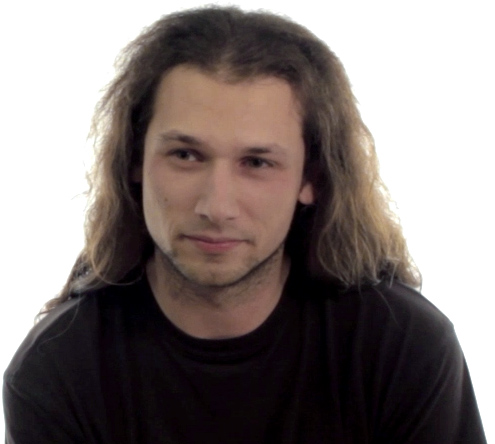
\includegraphics[width=\textwidth]{img/foto}
}

\emph{In a nuthsell} $\cdot$  Recent university graduate passionate about
technology looking for a challenge and an opportunity to learn
a new language.  Specialties include Real-Time Linux and software development.

\section*{Personal Information}

\standardEntry{Full name}{Jorge Manuel Coelho Amado de Azevedo}
\standardEntry{Address}{Rua Bartolomeu Dias, 210, 4450-587 Matosinhos,
Portugal}
\standardEntry{Date of Birth}{15th October 1987} 
\standardEntry{Age}{25}
\standardEntry{Gender}{Male} 
\standardEntry{Nationality}{Portuguese} 
\standardEntry{Telephone}{(+351) 936270876}
\standardEntry{E-mail}{jorge.amado.azevedo@gmail.com} 
\standardEntry{LinkedIn}{pt.linkedin.com/in/jaazevedo}
\standardEntry{Xing}{Jorge Azevedo}

\section*{Experience}

\stretchedEntry{UNISOL}{Universidade de Aveiro, Portugal}
\indentedEntry{Mar 2012 - Present}{\textbf{Researcher}}
\indentedEntry{Description}
{
Research grant for the UNISOL project.

Development of datalogging infrastructure.

Embedded control system prototype.

Deployment and admnistration of a MATLAB computational cluster, OpenStack cloud
computing environment.
}

\stretchedEntry{Xenomai Lab}{www.xenomailab.org}
\indentedEntry{Jan 2011 - Present}{\textbf{Software Engineer}}
\indentedEntry{Description}
{
Principal developer and maintainer of the Xenomai Lab platform.
}
\indentedEntry{Jan 2012 - Present}{\textbf{Master Thesis Colaborator}}
\indentedEntry{Description}{
Technical coordinator for several student master thesis

Sep 2012 - Present

TODO.

Jan 2012 - Dez 2012

"Adaptive Control Algorithms using Xenomai Lab".
}

\section*{Publications}

\standardEntry{September 2012}{Xenomai Lab - A Platform for Digital Real-Time Control}
\standardEntry{In}{INFORUM 2012 Procedings}

\section*{Education}

\standardEntry{2005–2012}{\textbf{M.Sc. Electronics and Telecommunications
Engineering}}
\standardEntry{Institution}
{
\textbf{Universidade de Aveiro}

Campus Universitário de Santiago, 3810-193 Aveiro, Portugal
}
\standardEntry{Thesis}{Xenomai Lab - A Platform For Digital Real-Time Control}
\standardEntry{Description}
{
5 year degree (Bachelor and Master's included).

Thesis graded 19/20 after public defense. 
}

\vspace{\baselineskip}

\standardEntry{2008–2009}{\textbf{Erasmus Exchange Program}}
\standardEntry{Institution}
{
\textbf{TU\textbackslash e Technische Universiteit Eindhoven}

Den Dolech 2, 5612 AZ Eindhoven, Netherlands
}
\standardEntry{Description}
{
One year spent abroad under the Erasmus Exchange Program.
}

\section*{Languages}

\standardEntry{Portuguese}{Native speaker}
\standardEntry{English}
{
Advanced speaker. Five years of education in the British Council achieving
level A in First Certificate of English (2001) and level B in Certificate of
Advanced English (2004)
}
\standardEntry{Spanish}{Basic understanding in both written and spoken form.}


\section*{Technical Skills}

\standardEntry{Programming}
{
Advanced knowledge of C.
			
Medium knowledge of C++, Java and the Android platform, Qt framework for GUI
programming/design, Linux kernel modules and filesystems.
			
Basic knowledge of Python, Objective C and iOS, Pascal, BASH scripting, VHDL,
MIPS and x86 Assembly assembly language.
}
\standardEntry{Electronics}
{
Medium Knowledge and hands-on experience with SPICE circuit simulation, Analog
and Digital filter design, Microcontrollers.
			 
Basic knowledge of Digital circuit design and circuit layout.

Extensive hands-on experience with circuit prototyping and signal analysis.
}
\standardEntry{General}
{
Advanced use of Microsoft Windows and Linux Operating Systems.

Extensive experience with Linux real-time variants, such as Xenomai and RTAI.

Word processing, spreadsheets and presentations with Microsoft Office, Open
Office and \LaTeX.

Basic experience with administrating Windows and Linux systems and networks.

Basic knowledge of classic and modern control engineering
}


\section*{Soft Skills}

\standardEntry{Social Skills}
{
Experience in multicultural environments

Open-Minded

Highly responsible and professional
}
\standardEntry{Organizational Skills}
{
Independent research

Strong drive for initiative

Planning and scheduling of team/individual project.
}

\section*{Additional Skills}

\standardEntry{Driving License}{Category B-1}

\end{document}
